% !TEX engine = lualatex
\documentclass[aspectratio=169]{divoc}

%%%%%%%%%%%%%%%%%%%%%
% PAQUETES
%%%%%%%%%%%%%%%%%%%%%

\setdefaultlanguage{english}
\setotherlanguage[variant=austrian]{german}
\usepackage[german]{datetime2}
\usepackage{subcaption}
\usepackage{siunitx}
\usepackage{emoji}
\sisetup{mode=text, per-mode=symbol}
\captionsetup[subfigure]{justification=centering}

%%%%%%%%%%%%%%%%%%%%%
% TEMPLATE
%%%%%%%%%%%%%%%%%%%%%
% Title graphics: BG + logo of the conference
\titlegraphic{
  \begin{tikzpicture}[remember picture, overlay]
    \scoped[on background layer]\node [centered,opacity=0.4] at (current page.center) {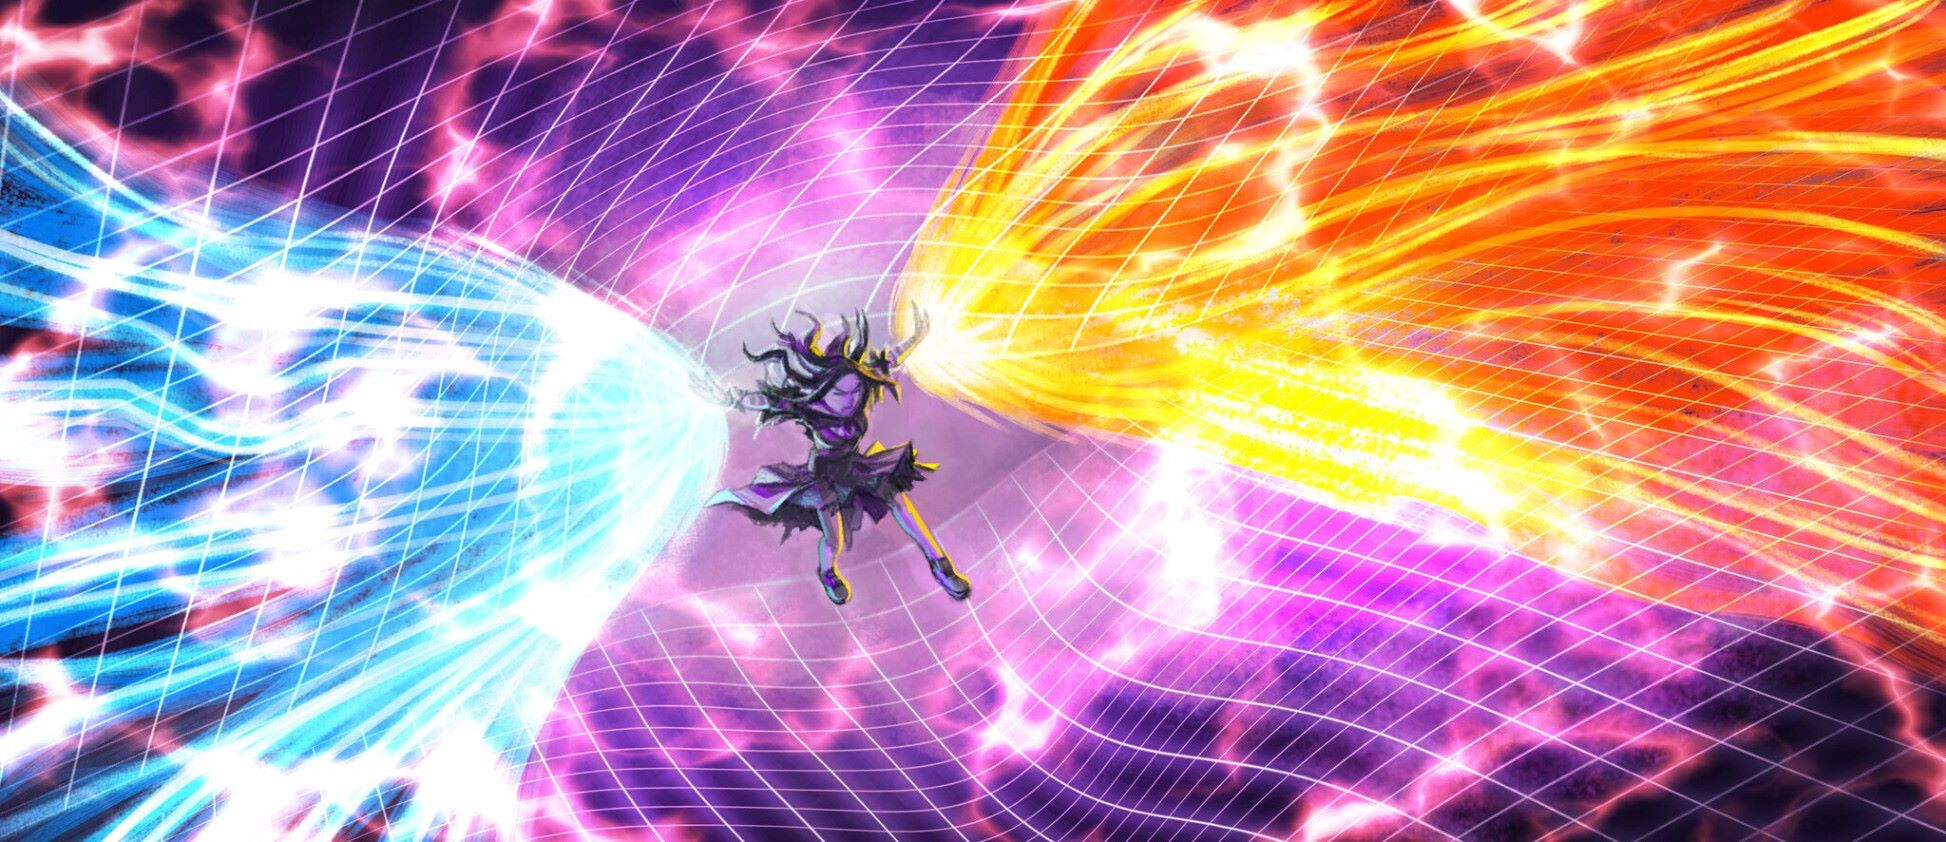
\includegraphics[width=\pagewidth,height=\pageheight]{frontmatter/5652946655be9e42.jpeg}};
    \scoped[on background layer]\node [above left] at (current page.south east) {
\includegraphics[height=4em,keepaspectratio]{frontmatter/annie-shenanigans}};
    \scoped[on background layer]\node [above right,align=left,font=\tiny\itshape] at (current page.south west) {
      Background: \href{https://framapiaf.org/@davidrevoy/104400422779912978}{David Revoy on Framapiaf} \\
      Seal: \href{https://lethalbit.net}{Aki Van Ness}, CC-BY-SA-4.0
    };
  \end{tikzpicture}
}

%%%%%%%%%%%%%%%%%%
% METADATA
%%%%%%%%%%%%%%%%%%

\title{The Curse of Slide-making}
\author{amyspark}
% \institute{Stitching Krita Foundation, Deventer, the Netherlands}
\date{\DTMdate{2022-04-17}}

\addbibresource{bibliography.bib}

\begin{document}
\maketitle

\begin{frame}{About me}
  \begin{itemize}[<*>]
    \item Full-time contract dev for KDE's Krita
    \item Colour spaces, SIMD, build systems... curses are my specialty \emoji{woman-mage}
    \item Occasional contributor to a lot of projects
    \item \href{https://www.amyspark.me}{amyspark.me}
  \end{itemize}
\end{frame}
\begin{frame}{Scope}
  \tableofcontents
\end{frame}
\section{Motivation}
\begin{frame}{Motivation}
  \begin{center}
    \enquote{I'll give a talk at \texttt{\$con}!}

    I can do it, right?
  \end{center}
\end{frame}
\begin{frame}{Motivation}
  \begin{itemize}
    \item Slide decks are a key tool in a lot of jobs
    \item Very specific topic
    \item (Sometimes) very tight deadline
    \item Reasonably long speaking time
  \end{itemize}
\end{frame}
\begin{frame}
  \begin{center}
    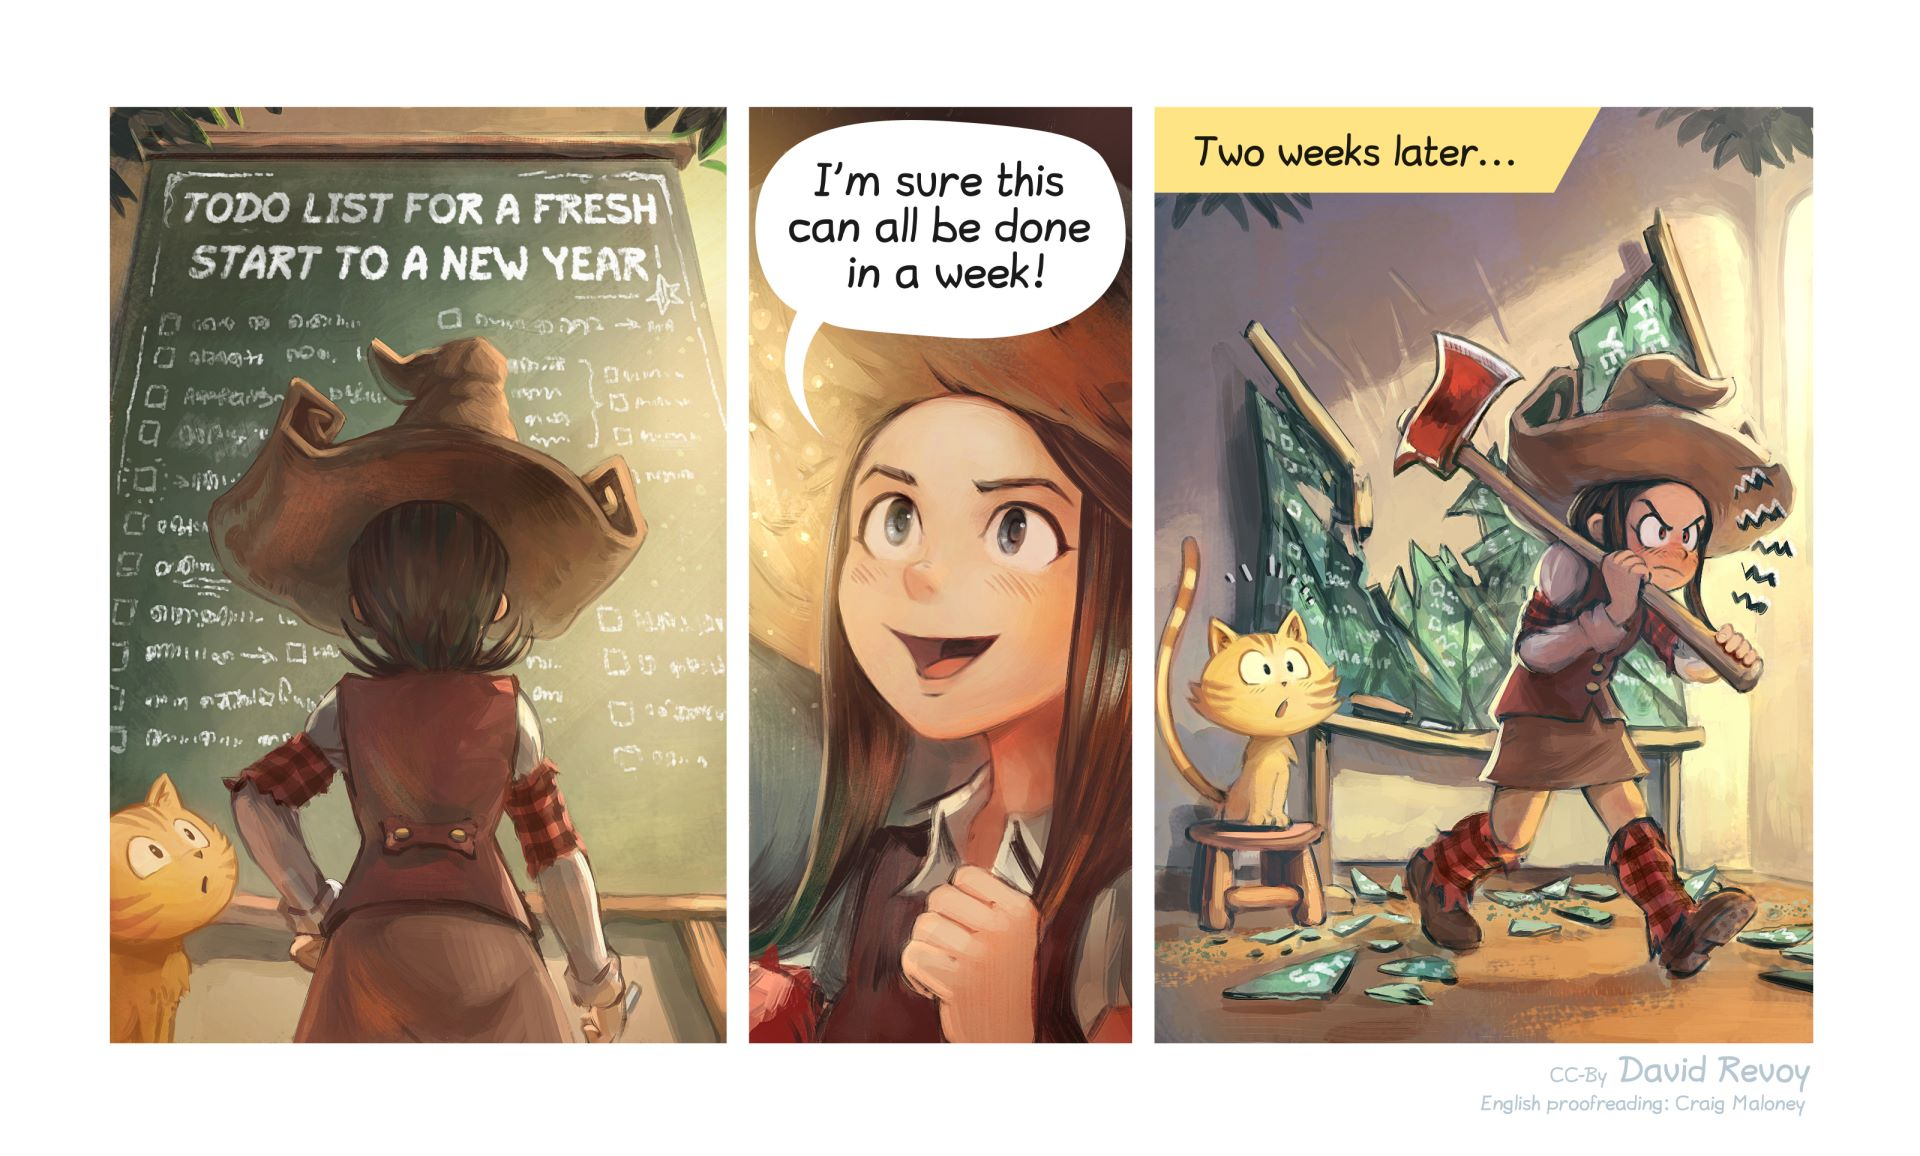
\includegraphics[width=\textwidth,keepaspectratio]{figures/2022-01-14_Strip-Comic_The-TODO-List_by-David-Revoy.jpg}
  \end{center}
\end{frame}
\begin{frame}{Motivation}
  \begin{itemize}
    \item Technical knowhow is important
    \item But the tool you choose is \emph{essential}
    \item It can make a difference for your presentation
    \item Know the pitfalls, don't suffer them later
  \end{itemize}
\end{frame}
\section{Requirements}
\begin{frame}{Requirements}
  They depend on a lot of things:
  \begin{itemize}
    \item organizational environment
    \item company/university requirements
    \item purpose of the talk
    \item available time
    \item intended/possible audience
    \item ...
  \end{itemize}
\end{frame}
\begin{frame}{Example}
  These are the requirements that my uni has for job interviews:

  \begin{itemize}
    \item Automagic templating/layout/styling
          \begin{itemize}
            \item each place/con can set its own guidelines
            \item automating saves spoons
          \end{itemize}
    \item Bibliography
          \begin{itemize}
            \item audience will want references
            \item I prefer putting these on slides
          \end{itemize}
    \item Mathematical tools
          \begin{itemize}
            \item we use these a lot in CS academia
          \end{itemize}
    \item Graphic making
          \begin{itemize}
            \item everyone wants at least a figure, right? \emoji{winking-face}
          \end{itemize}
  \end{itemize}
\end{frame}
\section{Tools}
\begin{frame}{Intro}
  Next slides will showcase a few of the tools I've tried.

  \begin{itemize}
    \item Pros
    \item Cons
    \item How they match (or not) the requirements
  \end{itemize}
\end{frame}
\begin{frame}{Tool \#1: your favourite presentation program}
  \begin{center}
    PowerPoint / LibreOffice Impress / Apple Keynote
  \end{center}

  Pros:
  \begin{itemize}
    \item Well-known, possibly also the most at-hand
    \item Assorted graphics options (though usually business-related)
    \item Portability
  \end{itemize}
\end{frame}
\begin{frame}{Tool \#1: your favourite presentation program}
  \begin{center}
    PowerPoint / LibreOffice Impress / Apple Keynote
  \end{center}

  Cons:
  \begin{itemize}
    \item Compatibility and budgets
          \begin{itemize}
            \item L-O is free, but still has compatibility issues
            \item Keynote is free w/Mac, but also the above
            \item PowerPoint is the reference software, but costs \euro\euro\euro
          \end{itemize}
    \item Lacks functionality for academic environments
          \begin{itemize}
            \item bibliography, equations, references
          \end{itemize}
    \item Graphic making is limited to the available options
    \item Ever tried styling a PowerPoint template?
  \end{itemize}
\end{frame}
\begin{frame}{Tool \#2: Online presentation tools}
  \begin{center}
    Google Slides, Prezi, Cryptpad, Reveal.js...
  \end{center}

  Pros:
  \begin{itemize}
    \item Ultra-portable, they run in any browser
    \item Collaborative editing
    \item Embedding online resources is a no-brainer
  \end{itemize}
\end{frame}
\begin{frame}{Tool \#2: Online presentation tools}
  \begin{center}
    Google Slides, Prezi, Cryptpad, Reveal.js...
  \end{center}

  Cons:
  \begin{itemize}
    \item They also lack tools for academia
          \begin{itemize}
            \item bibliography, equations, references
          \end{itemize}
    \item Graphic making is more limited than in desktop programs
    \item Styling choices are usually more constrained
    \item Extensibility is very limited (or none at all)
    \item GDPR concerns
  \end{itemize}
\end{frame}
\begin{frame}{Tool \#3: Pandoc}
  \begin{center}
    Pandoc is the \enquote{swiss army knife} for format transformation.
  \end{center}

  Pros:
  \begin{itemize}
    \item Write Markdown, render in just about \emph{any} format
    \item Bibliography and equations are included!
          \begin{itemize}
            \item (depending on the output format, but usually you can just render it)
          \end{itemize}
    \item A well made template removes you from the styling equation \emoji{tada}
  \end{itemize}
\end{frame}
\begin{frame}{Tool \#3: Pandoc}
  \begin{center}
    Pandoc is the \enquote{swiss army knife} for format transformation.
  \end{center}

  Cons:

  \begin{itemize}
    \item Templating is \emph{very} hard
    \item It often replicates the weirdness of the chosen output format
    \item If targeting LaTeX, you are probably duplicating work *and* toolchains
    \item Little control over bibliography formatting/splitting
          \begin{itemize}
            \item e.g. splitting bibliography across slides
            \item LaTeX + CSL is just not possible
          \end{itemize}
    \item Graphics are just \emph{impossible}
          \begin{itemize}
            \item at least in my experience?
          \end{itemize}
  \end{itemize}
\end{frame}
\begin{frame}{Tool \#4: Beamer}
  \begin{center}
    Beamer is a package for the LaTeX typesetting system.
  \end{center}

  Pros:
  \begin{itemize}
    \item Probably your tool of choice if you've already been exposed
          \begin{itemize}
            \item we use LaTeX a \emph{lot} in academia
          \end{itemize}
    \item It's what you are looking at now!
    \item Native bibliography handling
    \item Very extensible via hooks and package overrides
    \item PDF output (course notes, draft, slides...)
  \end{itemize}
\end{frame}

\begin{frame}{Tool \#4: Beamer}
  \begin{center}
    Beamer is a package for the LaTeX typesetting system.
  \end{center}

  Cons:
  \begin{itemize}
    \item Making graphics is baaaaaaaaaaaaaaaaaaaaaaaaaad
          \begin{itemize}
            \item This is probably its weakest point
            \item In my own case, it cost me many university job applications
          \end{itemize}
    \item As with anything LaTeX, it has a steep learning curve
          \begin{itemize}
            \item On its defence, it amortizes quickly over time
            \item For instance, this presentation was done with my thesis template, and I customized it for DiVOC with a few lines
          \end{itemize}
    \item You're also kind of limited to the hooks that Beamer (or your template) provide
          \begin{itemize}
            \item but if you know LaTeX, anything is possible \emoji{smile}
          \end{itemize}
  \end{itemize}
\end{frame}
\section*{Conclusions}
\begin{frame}{We covered}
  \begin{itemize}
    \item My motivation for the talk
    \item Requirements
    \item Tools showcase
  \end{itemize}
\end{frame}
\begin{frame}{Remarks}
  \begin{itemize}
    \item The weakest points of all tools are
          \begin{itemize}
            \item bibliography
            \item graphic making
          \end{itemize}
    \item Conclusion: don't reinvent the wheel
          \begin{itemize}
            \item if you have one, try extending it
            \item but I'd really wish for graphics to be easier
          \end{itemize}
  \end{itemize}
\end{frame}
\begin{frame}{Thank you for watching!}
  \begin{center}
    {
      \large
      \textbf{Got any questions or comments?}
    }
    \begin{itemize}[<*>]
      \item Q+A next
      \item Email: \href{mailto:amy@amyspark.me?subject="DiVOC 2022"}{amy@amyspark.me}
      \item Matrix: \href{https://matrix.to/\#/@amyspark:fairydust.space}{@amyspark:fairydust.space}
    \end{itemize}
  \end{center}
\end{frame}
\end{document}
